

\documentclass[11pt, a4paper, oneside]{Thesis} % Paper size, default font size and one-sided paper

\graphicspath{{./Pictures/}} % Specifies the directory where pictures are stored

\usepackage[square, numbers, comma, sort&compress]{natbib} % Use the natbib reference package - read up on this to edit the reference style; if you want text (e.g. Smith et al., 2012) for the in-text references (instead of numbers), remove 'numbers'
\usepackage{alltt} 
\hypersetup{urlcolor=black, colorlinks=true} % Colors hyperlinks in blue - change to black if annoying
\title{\ttitle} % Defines the thesis title - don't touch this

\begin{document}

\frontmatter % Use roman page numbering style (i, ii, iii, iv...) for the pre-content pages

\setstretch{1.3} % Line spacing of 1.3

% Define the page headers using the FancyHdr package and set up for one-sided printing
\fancyhead{} % Clears all page headers and footers
\rhead{\thepage} % Sets the right side header to show the page number
\lhead{} % Clears the left side page header

\pagestyle{fancy} % Finally, use the "fancy" page style to implement the FancyHdr headers

\newcommand{\HRule}{\rule{\linewidth}{0.5mm}} % New command to make the lines in the title page

% PDF meta-data
\hypersetup{pdftitle={\ttitle}}
\hypersetup{pdfsubject=\subjectname}
\hypersetup{pdfauthor=\authornames}
\hypersetup{pdfkeywords=\keywordnames}

%----------------------------------------------------------------------------------------
%	TITLE PAGE
%----------------------------------------------------------------------------------------

\begin{titlepage}
\begin{center}

\textsc{\LARGE \univname}\\[1.5cm] % University name

\includegraphics[scale=1]{logo1.jpg}\\
\textsc{\Large Lucrare de licen\c t\v a}\\[0.5cm] % Thesis type

\HRule \\[0.4cm] % Horizontal line
{\huge \bfseries \ttitle}\\[0.4cm] % Thesis title
\HRule \\[1.5cm] % Horizontal line
 
\begin{minipage}{0.4\textwidth}
\begin{flushleft} \large
\emph{Autor:}\\
{\authornames} % Author name - remove the \href bracket to remove the link
\end{flushleft}
\end{minipage}
\begin{minipage}{0.4\textwidth}
\begin{flushright} \large
\emph{\^Indrumator:} \\
\href{http://math.univ-ovidius.ro/default.aspx?cat=Personal&ItemID=37}{\supname} % Supervisor name - remove the \href bracket to remove the link  
\end{flushright}
\end{minipage}\\[3cm]
 
\large \textit{O lucrare creat\v a in scopul ob\c tinerii cerin\c telor\\ pentru ob\c tinerea diplomei de \degreename}\\[0.3cm] % University requirement text
\textit{\^in domeniul}
\deptname\\[2cm] % Research group name and department name
 
\textbf{Iunie 2013} % Date
%\includegraphics{Logo} % University/department logo - uncomment to place it
 %
\includegraphics[scale=1]{logo1.jpg} 
\vfill
\end{center}

\end{titlepage}

%----------------------------------------------------------------------------------------
%	DECLARATION PAGE
%	Your institution may give you a different text to place here
%----------------------------------------------------------------------------------------

%\Declaration{

%\addtocontents{toc}{\vspace{1em}} % Add a gap in the Contents, for aesthetics

%Eu, \authornames ,declar ca lucrarea de licen\c ta cu titlul  , '\ttitle' si munca prezentat\v a \^in %ea \^imi apar\c tin. Confirm ca:

%\begin{itemize} 
%\item[\tiny{$\blacksquare$}] This work was done wholly or mainly while in candidature for a research degree at this University.
%\item[\tiny{$\blacksquare$}] Where any part of this thesis has previously been submitted for a degree %or any other qualification at this University or any other institution, this has been clearly stated.
%\item[\tiny{$\blacksquare$}] Where I have consulted the published work of others, this is always %clearly attributed.
%\item[\tiny{$\blacksquare$}] Where I have quoted from the work of others, the source is always given. %With the exception of such quotations, this thesis is entirely my own work.
%\item[\tiny{$\blacksquare$}] I have acknowledged all main sources of help.
%\item[\tiny{$\blacksquare$}] Where the thesis is based on work done by myself jointly with others, I %have made clear exactly what was done by others and what I have contributed myself.\\
%\end{itemize}
 
%Signed:\\
%\rule[1em]{25em}{0.5pt} % This prints a line for the signature
 
%Date:\\
%\rule[1em]{25em}{0.5pt} % This prints a line to write the date
%}

%\clearpage % Start a new page

%----------------------------------------------------------------------------------------
%	QUOTATION PAGE
%----------------------------------------------------------------------------------------

\pagestyle{empty} % No headers or footers for the following pages

\null\vfill % Add some space to move the quote down the page a bit

\textit{``Thanks to my solid academic training, today I can write hundreds of words on virtually any topic without possessing a shred of information, which is how I got a good job in journalism."}

\begin{flushright}
Dave Barry
\end{flushright}

\vfill\vfill\vfill\vfill\vfill\vfill\null % Add some space at the bottom to position the quote just right

\clearpage % Start a new page

%----------------------------------------------------------------------------------------
%	ABSTRACT PAGE
%----------------------------------------------------------------------------------------

\addtotoc{Titlu} % Add the "Abstract" page entry to the Contents

\abstract{\addtocontents{toc}{\vspace{1em}} % Add a gap in the Contents, for aesthetics


}

\clearpage % Start a new page

%----------------------------------------------------------------------------------------
%	ACKNOWLEDGEMENTS
%----------------------------------------------------------------------------------------
\renewcommand{\bibname}{Bibliografie}
\renewcommand{\listfigurename}{List\v a imagini}
\renewcommand{\contentsname}{Cuprins}
\setstretch{1.3} % Reset the line-spacing to 1.3 for body text (if it has changed)

\acknowledgements{\addtocontents{toc}{\vspace{1em}} % Add a gap in the Contents, for aesthetics

The acknowledgements and the people to thank go here, don't forget to include your project advisor\ldots
}
\clearpage % Start a new page

%----------------------------------------------------------------------------------------
%	THESIS CONTENT - CHAPTERS
%----------------------------------------------------------------------------------------

\pagestyle{fancy} % The page style headers have been "empty" all this time, now use the "fancy" headers as defined before to bring them back

\lhead{\emph{Contents}} % Set the left side page header to "Contents"
\tableofcontents % Write out the Table of Contents

%----------------------------------------------------------------------------------------
%	DEDICATION
%----------------------------------------------------------------------------------------

%\setstretch{1.3} % Return the line spacing back to 1.3

%\pagestyle{empty} % Page style needs to be empty for this page

%\dedicatory{For/Dedicated to/To my\ldots} % Dedication text

%\addtocontents{toc}{\vspace{2em}} % Add a gap in the Contents, for aesthetics

%----------------------------------------------------------------------------------------
%	THESIS CONTENT - CHAPTERS
%----------------------------------------------------------------------------------------

\mainmatter % Begin numeric (1,2,3...) page numbering

\pagestyle{fancy} % Return the page headers back to the "fancy" style

% Include the chapters of the thesis as separate files from the Chapters folder
% Uncomment the lines as you write the chapters
\renewcommand{\chaptername}{Capitolul}
% Chapter 1

\chapter{Introducere} % Main chapter title

\label{Chapter1} % For referencing the chapter elsewhere, use \ref{Chapter1} 

\lhead{Capitolul 1. \emph{Teoria compilarii}} % This is for the header on each page - perhaps a shortened title

%----------------------------------------------------------------------------------------

\section{De ce teoria compilarii}
	Prima oara cand am auzit despre ce inseamna un compilator a fost in liceu cand am invatat despre
	limbajul de programare Pascal.De atuncti pana in prezent am invatat o multime de alte limbaje.Cu 
	toate acestea nu stim cu adevarat ce inseamna un limbaj de programare desi pe unele dintre ele
	stiam sa le folosesc.Desi aveam cunostinte de limbaje formale tot nu puteam sa imi dau seama cum
	sunt imbinate acele modele matematice (gramatici,automatele finite) intr-o aplicatie care sa 
	generez cod.
	
		
	
	

%----------------------------------------------------------------------------------------



%Chapter 2
\chapter{Preliminare}%informatii despre teoria limbajelor formale -pe scurt info despre automate finite si metode de transformare a gramaticilor
\label{Chapter2}
\lhead{Capitolul 2. \emph{Preliminare}}
\begin{quotation}


 Fie T o mul\c time de simboluri denumit\v a alfabet. Orice submul\c time a mul\c timii $T^{*}$ reprezint\v a un limbaj asupra alfabetului T. Elementele limbajului se numesc propozi\c tii. Dac\v a limbajul este finit atunci el poate s\v a fie definit prin enumerare. De exemplu consider\^ and alfabetul B = $\lbrace$ 0, 1 $\rbrace$ atunci L = $\lbrace$01, 10, 101 $\rbrace$ este un limbaj. Mul\c timea cuvintelor din limbajul natural este \c si el un limbaj pentru care se poate pune problema enumer\v arii tuturor cuvintelor, chiar dac\v a lista care ar rezulta este imens\v a, deci este un limbaj reprezentabil prin enumerare. Dar cazul interesant este cel \^n care limbajul este infinit. S\v a consider\v am de
exemplu limbajul "\c sirurilor formate din 0 \c si 1 a c\v aror lungime este divizibil\v a cu 3". Evident este vorba de un limbaj infinit. Textul prin care am specificat limbajul constituie o reprezentare finit\v a a limbajului. Nu este singura solu\c tie posibil\v a de reprezentare finit\v a. De exemplu dac\v a notam cu L limbajul respectiv atunci:  
$$ L = \lbrace w \in \lbrace0,1 \rbrace^{*} \slash |w| mod 3 = 0 \rbrace$$
este un alt mod de a specifica acela\c si limbaj. 
\end{quotation}
\begin{quotation}
 \^ In general exist\v a doua mecanisme distincte de definire finit\v a a limbajelor: prin generare sau prin recunoa\c stere. \^In primul caz este vorba de un "dispozitiv" care \c stie s\v a genereze toate propozi\c tiile din limbaj (\c si numai pe acestea) astfel \^inc\^ at aleg\^ and orice propozi\c tie din limbaj \^ intr-un interval finit de timp dispozitivul va ajunge să genereze propozi\c tia respectiv\v a. \^ In al doilea caz este vorba de un "dispozitiv" care \c stie s\v a recunoasc\v a (s\v a accepte ca fiind corecte) propozi\c tiile limbajului dat. 
\end{quotation}

\section{Gramatici}
\begin{quotation}
%O gramatica Chomsky este o constructie: G=(N,T,P,S) unde: N=multimea finita de neterminali,T=multime %finita de "terminali" :$N\cap T=\emptyset,S\in N $=este simbolul de "start" si $P\subseteq(N\cup %T)^{*}N(N\cup T)^{*}\times(N\cup T)^{*}$ este o multime finita de productii.
 O gramatic\v a reprezint\v a cel mai important exemplu de generator de limbaje. Prin defini\c tie o gramatic\v a este G = (N, T, P, S) unde :
 \begin{itemize}
 \item {N este o mulţime finită de simboli numită mulţimea simbolilor neterminali;}
 \item {T este o mul\c time finit\v a de simboli numit\v a mul\c timea simbolilor terminali,($N\cap T=\emptyset$);}
 \item {P este o submul\c time finit\v a din $(N\cup T)^{*}N(N\cup T)^{*}\times(N\cup T)^{*} $;numit\v a mul\c timea produc\c tiilor gramaticii. Un element $(\alpha,\beta)\in P$ este notat cu $\alpha \rightarrow \beta$ \c si se nume\c ste produc\c tie.  
 }
 \item {$S \in N $ este un simbol special numit simbol de start al gramaticii G.}

\end{itemize}  
\end{quotation}
\subsection{Transform\v ari asupra gramaticilor independente de context}
\begin{quotation}
Din punctul de vedere al procesului de compilare, gramaticile sunt utilizate pentru faza de analiz\v a 
sintactic\v a, pentru care se utilizeaz\v a gramatici independente de context. Exist\v a o serie de metode de analiza sintactic\v a, bine puse la punct at\^ at din punct de vedere teoretic c\^ at şi practic. Fiecare dintre aceste metode impune \^ins\v a o serie de restric\c tii asupra gramaticilor utilizate. \^In general atunci c\^ and se construie\c ste o gramatic\v a se pleac\v a de la forma general\v a a structurilor pe care aceasta trebuie s\v a le descrie \c si nu de la metoda de analiz\v a sintactic\v a ce va fi utilizat\v a. \^In acest mod se ob\c tine o gramatic\v a ce poate să fie "citit\v a" u\c sor de c\v atre proiectant. Pentru a satisface \^ ins\v a condi\c tiile impuse de c\v atre metodele de analiz\v a sintactic\v a sau de c\v atre generarea de cod, se realizeaz\v a transform\v ari asupra gramaticilor. Aceste transform\v ari trebuie s\v a p\v astreze neschimbat limbajul generat. \^In cele ce urmeaz\v a vom prezenta c\^ ateva transform\v ari tipice asupra gramaticilor independente de context. Pentru a explica semnifica\c tia acestor transform\v ari \^ in contextul analizei sintactice vom prezenta \^ int\^ ai no\c tiunea de arbore de derivare. 
\end{quotation}
\begin{quotation}
 Un arbore de derivare este o reprezentare grafic\v a pentru o secven\c t\v a de deriv\v ari (de aplic\v ari ale rela\c tiei $\Rightarrow$ \^ intre formele propozi\c tionale). \^ Intr-un arbore de derivare nu se mai poate identifica ordinea \^ in care s-a  f\v acut substitu\c tia simbolilor neterminali. Fiecare nod interior arborelui, reprezint\v a un neterminal.Descenden\c tii unui nod etichetat cu un neterminal A sunt eticheta\c ti de la st\^ anga la dreapta prin simbolii care formeaz\v a partea dreapt\v a a unei produc\c tii care are \^ in partea st\^ anga neterminalul A. Parcurg\^ and de la st\^ anga la dreapta frunzele unui astfel de arbore se ob\c tine o form\v a propozi\c tional\v a. S\v a consider\v am de exemplu din nou gramatica \c sirurilor de paranteze bine formate:\\
$  G = (\lbrace S \rbrace, \lbrace(,)\rbrace, \lbrace S → (S)S \vert \lambda \rbrace, S)$ \\
Fie urm\v atoarea secven\c t\v a de deriv\v ari:\\
$ S \Rightarrow ( S ) S \Rightarrow ( ( S ) S ) S \Rightarrow ( () S ) S \Rightarrow 
 ( () ( S ) S ) S \Rightarrow ( () () S ) S \Rightarrow 
 ( () () ) S \Rightarrow ( () () ) ( S ) S \Rightarrow^{*}( ()() ) ()$\\
 Se ob\c tine arborele de derivare:\\
 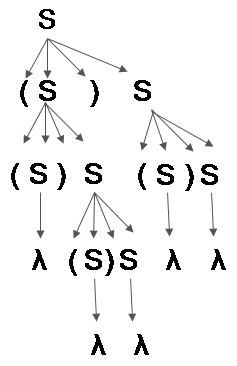
\includegraphics{arbore1.png}
 \label{arbore1}
\end{quotation}
\subsection{Eliminarea ambiguit\v a\c tii}
O gramatic\v a care produce mai mul\c ti arbori de derivare pentru aceea\c si propozi\c tie este o gramatic\v a 
ambigu\v a. Deoarece exist\v a tehnici de analiz\v a sintactic\v a care lucreaz\v a numai cu gramatici neambigue vom \^ incerca s\v a construim gramatici care genereaz\v a acela\c si limbaj \c si care sunt neambigue.  S\v a consider\v am de exemplu urm\v atoarea gramatic\v a: 
\begin{verbatim}
instr → if expresie then instr | 
 if expresie then instr else instr |
 alte_instr 
\end{verbatim}
S\v a construim arborele de derivare pentru propozi\c tia : 
\begin{verbatim}
if E1 then if E2 then S1 else S2
\end{verbatim}

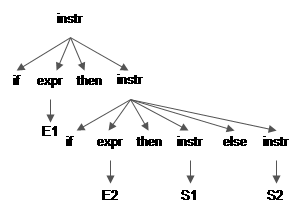
\includegraphics[scale=1]{arbore2.png}
\\
Pentru aceast\v a propozi\c tie mai exist\v a \^ins\v a un arbore de derivare.
\\
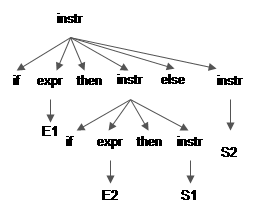
\includegraphics[scale=1]{arbore3.png}

\paragraph*{}
\^In toate limbajele de programare care accept\v a construc\c tii de tip if then else se consider\v a cu sens prima derivare \^ in care fiecare clauza else este atribuit\v a instruc\c tiunii if cea mai interioar\v a. Rezult\v a deci condi\c tia pe care trebuie s\v a o satisfac\v a o instruc\c tiune if. Instruc\c tiunea cuprins\v a \^ intre then \c si else trebuie s\v a nu fie o instruc\c tiune if sau s\v a fie o instruc\c tiune if cu clauza else. Rezult\v a urm\v atoarea gramatic\v a ob\c tinut\v a prin
transformarea gramaticii anterioare: 
\begin{verbatim}
instr → if_cu_else| if_fara_else                               
  if_cu_else → if expresie then if_cu_else else if_cu_else |      
                alte_instr                                        
  if_fara_else → if expresie then instr |                         
                  if expresie then if_cu_else else if_fara_else 
\end{verbatim}

Se observ\v a c\v a aceast\v a gramatic\v a genereaz\v a acela\c si limbaj cu gramatica anterioar\v a dar accept\v a o derivare unic\v a pentru propozi\c tia : 
\begin{verbatim}
 if E1 then if E2 then S1 else S2 
\end{verbatim}
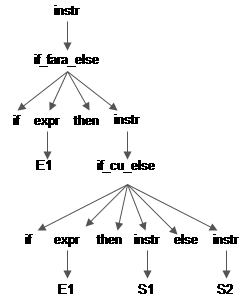
\includegraphics[scale=1]{arbore4.png}
\paragraph*{}
Se nume\c ste produc\c tie ambigu\v a o produc\c tie care are \^ in partea dreapt\v a mai multe apari\c tii ale aceluia\c si simbol neterminal.Existen\c ta unei produc\c tii ambigue nu implic\v a faptul că gramatica este ambigu\v a.
%______________________________________
%
%
%
%
%_______________________________________
\subsection{Eliminarea recursivit\v a\c tii st\^ anga }
\paragraph*{}
O gramatic\v a este recursiv\v a st\^ anga dac\v a exist\v a un neterminal A astfel \^ inc\^ at exist\v a o derivare A $\Rightarrow ^{*}$ A$\beta$
pentru $\beta \in(T \cup N)^{*}$. O analiz\v a sintactic\v a descendent\v a determinist\v a nu poate s\v a opereze cu o astfel de gramatic\v a, deci este necesar\v a o transformare.
S\v a consider\v am \^ int\^ ai cazul cel mai simplu pentru care \^ in
gramatic\v a exist\v a produc\c tii de forma $A \rightarrow A\beta | \alpha$. \^In acest caz limbajul generat este de forma $\alpha \beta$ cu n ≥ 0.
Acela\c si limbaj poate s\^ a fie generat de c\v atre gramatica: A → $\alpha$A', A' → $\beta$A'| $\lambda$. 
\\
 S\v a consider\v am de exemplu gramatica expresiilor aritmetice :\\
 $ E \rightarrow E + T | T, T \rightarrow T * F | F, F \rightarrow (E) | a $
\\
 Se observ\v a ca pentru un \c sir de forma a+a*a,examinand numai primul simbol terminal (a) nu este clar cu ce produc\c tie dintre produc\c tiile pentru E trebuie s\v a se \^inceap\v a derivarea.Aplic\^ and ideea anterioar\v a se ob\c tine:\\
$ E \rightarrow T E', E' \rightarrow +TE' | \lambda, T \rightarrow FT', T' \rightarrow *FT' | \lambda, F \rightarrow (E) | a $
\\
\^In acest caz derivarea va \^incepe sigur prin aplicarea produc\c tiei Ε → TE' \c si se ob\c tine derivarea Ε $\Rightarrow$ TE' $\Rightarrow$ FT'Ε'. \^In acest moment se vede c\v a pentru F trebuie s\v a se aplice produc\c tia F $\rightarrow$ a. Deci se ob\v tine Ε $\Rightarrow$ aT'Ε'. Urmeaz\v a simbolul terminal + datorit\v a c\v aruia pentru T' se va aplica produc\c tia T' → $\lambda$, etc. 
\paragraph*{}
Dac\v a gramatica nu permite deriv\v ari de tipul A $\Rightarrow ^{*}$ A (f\v ar\v a cicluri ) \c si nu con\c tine $\lambda$ - produc\c tii poate s\v a fie transformat\v a \^ in vederea elimin\v arii recursivit\v a\c tii st\^ anga utiliz\^ and urm\v atorul algoritm, ob\b tin\^ andu-se o gramatic\v a echivalent\v a f\v ar\v a recursivitate st\^ anga. 

\textit{
Se aranjeaz\v a neterminalele \^ in ordinea A1, ..., An\\
pentru i = 1 p\^ an\v a la n  executa \\
pentru j = 1 p\^ an\v a la i - 1 executa \\ 
\^inlocuie\c ste fiecare produc\c tie de forma $A_{i} \rightarrow A_{j} \beta$ cu produc\c tiile \\ $A_{i} \rightarrow → \alpha_{1}\beta | \alpha_{2}\beta|...|\alpha_{k}\beta  $ \\
unde $A_{j}\rightarrow \alpha_{1}|\alpha_{2}|\alpha_{3}|...|\alpha_{k}$\\
sunt toate produc\c tiile pentru $A_{j}$
\\
elimin\v a recursivitatea st\^ ang\v a \^ intre produc\c tiile $A_{i}$
}


%________________________________


\subsection{Factorizare st\^ anga}
\paragraph*{}
 Acest tip de transformare este util pentru producerea unei gramatici potrivite pentru analiza sintactic\v a 
descendent\v a de tip determinist. Ideea este că dac\v a nu este clar care dintre produc\c tiile alternative poate s\v a fie aplicat\v a pentru un neterminal se va am\^ ana luarea unei decizii p\^ an\v a c\^ and s-a parcurs suficient din \c sirul
de intrare pentru a se putea lua o decizie. S\v a consider\v am de exemplu produc\c tiile : \\
S $\rightarrow$ AbS $|$A \\
A $\rightarrow$ BcA $|$B \\
B $\rightarrow$ a $|$ dSd 
\paragraph*{}

S\v a presupunem c\v a \^ incerc\v am s\v a construim \c sirul deriv\v arilor pentru a b a c a pornind de la simbolul de start al gramaticii. Din recunoa\c sterea simbolului a la \^ inceputul \c sirului nu se poate \^ inc\v a trage concluzia care dintre cele doua produc\c tii corespunz\v atoare neterminalului S trebuie s\v a fie luata \^ in considerare (abia la \^ int\^ alnirea caracterului b pe \c sirul de intrare se poate face o alegere corect\v a). \^In general pentru produc\c tia $A \rightarrow \alpha \beta_{1} | \alpha \beta_{2}$ dac\v a se recunoa\c ste la intrare un \c sir nevid derivat din $\alpha$ nu se poate \c stii dac\v a trebuie aleas\v a prima sau a doua produc\c tie. Corespunz\v ator este util\v a transformarea: A $\rightarrow \alpha$ A', A'$\rightarrow \beta_{1}|\beta_{2}$. \\
 Algoritmul de factorizare func\c tioneaz\v a \^ in modul urm\v ator. Pentru fiecare neterminal A se caut\v a cel mai lung prefix $\alpha$ comun pentru dou\v a sau mai multe dintre produc\c tiile corespunz\v atoare neterminalului A. Dac\v a $\alpha\neq \lambda $ atunci se \^ inlocuiesc produc\c tiile de forma $A \rightarrow \alpha \beta_{1}$|$ \alpha \beta_{2}$| ... | $\alpha \beta_{n}$| $\delta$ (unde $\delta$ reprezint\v a alternativele care nu \^ incep cu $\alpha$) cu : \\
A $\rightarrow \alpha A' \delta$
A' $\rightarrow \beta_{1}|\beta_{2}|...|\beta_{n}$
A' este un nou neterminal. Se aplic\v a \^ in mod repetat aceast\v a transformare p\^ an\v a c\^ and nu mai exist\v a dou\v a alternative produc\c tii cu un prefix comun pentru acela\c si simbol neterminal.
 Relu\^ and exemplul considerat se ob\c tine :\\
      S $\rightarrow$ AX \\
     X $\rightarrow$ bS $|$ $\lambda$\\
     A $\rightarrow$ BY \\
     Y $\rightarrow$ cA $|$ $\lambda$\\
      B $\rightarrow$ a $|$ dSd \\

Deci \^ in analiza \c sirului a b a la \^int\^ alnirea simbolului b pentru neterminalul Y se va utiliza produc\c tia Y $\rightarrow$ $\lambda$, \^ in acest mod rezult\v a \c sirul de deriv\v ari :\\
   S $\Rightarrow$ AX $\Rightarrow$ BYX  $\Rightarrow$ aYX $\Rightarrow$ ... 
 

%________________________________________________________________________
%SECTIUNEA A DOUA ATOMATE FINITE
%________________________________________________________________________

\section{Automate finite}

Un automat finit este sistemul A=(Q,$\Sigma$,$\delta$,$q_{0}$,F) unde Q si F sunt nul\c timi,nevide, numite mul\c timea starilor respectiv \textit{ alfabetul de intrare}, $q_{0} \in Q $
este \textit{starea initiala},F$\subseteq$Q este \textit{multimea starilor finale} iar
$\delta$ este o func\c tie $\delta : Q x (\Sigma \cup {\varepsilon}) \rightarrow 2^{Q}$,
numita \textit{func\c tia de tranzi\c tie}
(unde prin $2^{Q}$ s-a notat mul\c timea par\c tilor lui Q).
\paragraph*{}
Modelul prezentat mai sus este cel cunoscut in literatura \c si sub denumirea de automat nedeterminist cu $\varepsilon$ - tranzi\c tii.
%adaug definitia automatului finit determinist
Un automat finit poate fi reprezentat prin \textit{tabela de tranzi\c tie} (func\c tia $\delta$) sau prin \textit{graful de tranzi\c tie}
\^In reprezentarea grafului de tranzi\c tie facem conven\c tia ca starile care nu sunt finale sa le reprezent\v am prin cercuri iar cele finale prin p\v atrate.De asemenea $\varepsilon$ -tranzi\c tiile sunt reprezentate prin arce neetichetate.
\textbf{Exemple de automate}\\
Fie Q=\{0,1,2 \} $\Sigma$ =\{a,b,c \} F=\{2\},$q_{0}$=0,iar $\delta$ este dat\v a astfel:

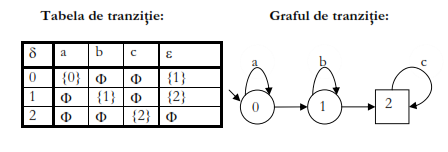
\includegraphics[scale=1]{exemplu_automat.png}


Fie Q=\{0,1,2 \},$\Sigma$=\{a,b \},
F=\{2 \},$q_{0}$=0,iar $\delta$ este:

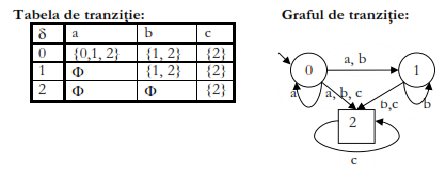
\includegraphics[scale=1]{exemplu_automat2.png}

\textbf{Definitie} Un automat A=(Q,$\Sigma$,$\delta$,$q_{0}$,F) se numeste:
\begin{enumerate}


\item{\textit{nedeterminist} (fara $\varepsilon$ - tranzitii),daca $\delta(q,\varepsilon)=\emptyset$,$\forall q \in Q$}
\item{\textit{determinist},dac\v a
$\delta(q,\varepsilon)=\emptyset$,$\forall q \in Q $ \c si $|\delta(q,a)|\leq 1$ , $\forall q \in Q$,$\forall a \in \Sigma$ 
 } 
\end{enumerate}
%______________________________________
% EXPRESII REGULATE
%______________________________________

\section{Expresii regulate}
Fie $\Sigma$ un alfabet, simbolurile $\varepsilon,\emptyset,|,\bullet,*,),($ care nu apar\c tin lui $\Sigma$ \c si E un cuv\^ ant peste alfabetul $\Sigma \cup \{\varepsilon,\emptyset,|,\bullet,*,),( \}$.O expresie regulat\v a peste $\Sigma$ se define\c ste inductiv astfel: \\
\begin{enumerate}
\item {
E este un \textit{atom regulat} peste $\Sigma$ daca E este un simbol $\Sigma \cup \{ \varepsilon,\emptyset \}$ sau este de forma ($E_{1}$) unde $E_{1}$ este o expresie regulata peste $\Sigma$;
}
\item{E este \textit{factor regulat} peste $\Sigma$ daca E este un atom regulat peste peste $\Sigma$ sau este de forma E1* unde $E_{1}$ este un factor regulat peste $\Sigma$}

\item{
E este un \textit{ termen regulat} peste $\Sigma$ dac\v a
E este un factor regulat peste $\Sigma$
sau este de forma $E_{1}\bullet E_{2}$
unde $E_{1}$ este un termen regulat, iar $E_{2}$ este un factor regulat peste $\Sigma$; 
}
\item{
E este o \textit{expresie regulat\v a} peste $\Sigma$ dac\v a E este un termen regulat peste $\Sigma$ sau este de forma $E_{1}| E_{2}$, unde $E_{1}$ este o expresie regulată, iar $E_{2}$ este un termen regulat peste
$\Sigma$. 
}
\end{enumerate}
Aici $\varepsilon,\emptyset$ sunt privite ca simple simboluri f\v ar\v a vreo semnifica\c tie. Mai jos, interpretarea acestor expresii va fi desigur limbajul \{$\varepsilon$ \} respectiv limbajul vid. 
 
%algoritimi de parsere ( ierarhia + informatii despre ei + gramaticile particulare (ex gramatica de expresii))
\chapter{Algoritmi de parsare}
\label{Chapter3}
\lhead{Capitolul 3. \emph{Algoritmi de parsare}}

\section{Problema pars\v arii}
Problema recunoa\c sterii \^ in gramatici independente de context este urm\v atoarea: Dat\v a o
gramatic\v a G = (V, T, S, P) \c si un cuv\^ ant w$\in T^{*}$, care este r\v aspunsul la \^ intrebarea w$\in$L(G)? Se
\c stie c\v a problema este decidabil\v a; mai mult, exist\v a algoritmi care \^ in timp O($|w|^{3}$) dau r\v aspunsul la \^ intrebare (Cooke-Younger-Kasami, Earley, vezi [Gri86]).
Problema pars\v arii(analizei sintactice) este problema recunoa\c sterii la care se adaug\v a: dac\v a r\v aspunsul la \^ intrebarea w$\in$L(G) este afirmativ, se cere arborele sintactic (o reprezentare
a sa) pentru w. 

%Fie G = (V, T, S, P) o gramatică
%şi w∈L(G). Să notăm prin $\overset{p}%{\underset{st}{\Rightarrow}}$
% ($\overset{q}{ \underset {dr} {\Rightarrow}}$) relaţia de derivare extrem stângă(dreaptă) în care, pentru rescriere s-a aplicat producţia p∈P (q∈P). 
\section{Analiza sintactic\v a descendent\v a}
Analiza sintactic\v a descendent\v a
(parsarea descendent\v a) poate fi considerat\v a ca o tentativ\v a
de determinare a unei deriv\v ari extrem st\^ angi pentru un cuv\^ ant de intrare. \^ In termenii arborilor sintactici, acest lucru \^ inseamn\v a tentativa de construire a unui arbore sintactic pentru cuv\^ antul de intrare, pornind de la r\v ad\v acin\v a \c si construind nodurile \^ in manier\v a descendent\v a, \^ in preordine (construirea r\v adacinii, a subarborelui st\^ ang apoi a celui drept).Pentru realizarea acestui fapt avem nevoie de urm\v atoarea structur\v a
(figura 3.1):
\begin{itemize}
\item
{
	o band\v a de intrare \^ in care se introduce cuv\^ antul de analizat, care se parcurge de la st\^ anga la dreapta, simbol cu simbol; 
}
\item
{
	o memorie de tip stiv\v a(pushdown) \^ in care se ob\c tin formele propozi\c tionale st\^ angi(\^ incep\^ and cu S). Prefixul formei propozi\c tionale format din terminali se compar\v a cu simbolurile curente din banda de intrare ob\c tin\^andu-se astfel criteriul de \^ inaintare \^ in aceast\v a band\v a; 
}
\item
{
	o band\v a de ie\c sire \^ in care se \^ inregistreaz\v a pe r\^ and produc\c tiile care s-au aplicat \^ in derivarea extrem st\^ ang\v a care se construie\c ste. 
}

\end{itemize}

\begin{figure}[htbp]
\centering
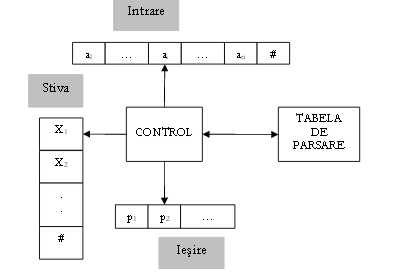
\includegraphics[scale=1]{parser_descendent.png}
	\rule{35em}{0.5pt}
\caption{Reprezentarea unui parser descendent}
	\label{fig:ParserDescendent}
\end{figure}

%\begin{figure}[htbp]
%	\centering
		%
\includegraphics{./Figures/Electron.pdf}
%		\rule{35em}{0.5pt}
%	\caption[An Electron]{An electron %(artist's impression).}
%	\label{fig:Electron}
%\end{figure}

Criteriul de oprire cu succes este acela \^ in care s-a parcurs \^ intreaga band\v a de intrare, iar memoria pushdown s-a golit. \^ In acest caz \^ in banda de ie\c sire s-a ob\c tinut parsarea st\^ ang\v a a cuv\^ antului respectiv. Iat\v a
un exemplu de cum func\c tioneaz\v a
acest mecanism (consider\v am
gramatica din exemplul precedent
\c si cuv\^ antul w = id+id*id). Vom considera caracterul \# pentru marcarea sf\^ ar\c sitului benzii de intrare (marca de sf\^ ar\c sit a cuv\^ antului) precum \c si pentru a marca baza stivei. 

\subsection{Gramaticile LL(1)}
Pentru ca un parser SLL(k) s\v a
poată fi implementat, trebuie s\v a
indic\v am o procedur\v a
pentru calculul mul\c timilor $FIRST_{k}$ \c si $FOLLOW_{k}$. Pentru c\v a \^ in practic\v a
se folose\c ste destul de rar (dac\v a nu chiar deloc) cazul k $\geq$ 2, vom restr\^ ange discu\c tia pentru cazul k=1. Vom nota \^ in acest caz $FIRST_{1}$ şi $FOLLOW_{1}$
prin FIRST respectiv FOLLOW.
A\c sadar, dac\v a
$\alpha\in \Sigma^{+}$, A$\in$V : \\
FIRST($\alpha$) = $\{a| a\in$T,$\alpha \overset{*}{\underset{st}{\Rightarrow}} au \}\cup$
if $(\alpha\overset{*}{\underset{st}{\Rightarrow}} \varepsilon)$ then ${\varepsilon}$ else $\emptyset$. \\
FOLLOW(A) = $\{a|a\in T \cup{\varepsilon}, S\overset{*}{\underset{st}{\Rightarrow}}uA\gamma$, $a\in FIRST (\gamma) \}$
Mai \^ int\^ ai s\v a ar\v at\v am c\v a gramaticile SLL(1) coincid cu gramaticile LL(1).  
\begin{theorem}
 O gramatic\v a G = (V, T, S, P) este gramatic\v a LL(1) dac\v a \c si numai dac\v a pentru orice $A \in V$ \c si pentru orice produc\c tii $A\rightarrow \beta_{1}|\beta_{2}$
are loc:
 \begin{flushleft}
 FIRST ($\beta_{1}$FOLLOW (A))$\cap$ 	FIRST($\beta_{2}$FOLLOW(A))=$\emptyset$
 \end{flushleft}

\end{theorem}
\subsection{Determinarea mul\c timilor FIRST \c si FOLLOW }
Vom indica \^ in acest paragraf modalitatea de determinare a mul\c timilor FIRST \c si FOLLOW pentru o gramatic\v a G.Un algoritm pentru determinarea mul\c timilor FIRST(X) este descris mai jos.\\
\textbf{Intrare:} Gramatica G=(V,T,S,P) redus\v a;\\
\textbf{Iesire:} FIRST(X),X$\in \Sigma$.\\
\textbf{Metoda:}Mul\c timile FIRST sunt completate prin inspectarea regulilor gramaticii\\
\begin{alltt}
1.for (X \(\in \Sigma\))
2.	if (X\( \in\)T) FIRST(X) = \({ X }\) else FIRST(X)=\(\emptyset\);
3.for (A \(\rightarrow \alpha \beta \in P\))
4.	FIRST (A) = FIRST(A) \(\cup\) \{ a \};
5.FLAG = true;
6.while(FLAG) \{ // FLAG marcheaza schimbarile in FIRST
7.	FLAG = false;
8.	for( \(A \rightarrow X1 X2 \ldots Xn \in P \)) \{
9.		i = 1;
10.     if((FIRST(X1)\(\nsubseteq\)FIRST(A)) \{
11.     	FIRST(A) = FIRST(A)\(\cup\)(FIRST(\(X1\));
12.			FLAG = true;
		\}//endif
13.		while(i<n && Xi\(\overset{+}{\underset{st}{\Rightarrow}}\)\(\varepsilon \) )
14.			if((FIRST(Xi+1)\( \nsubseteq \)FIRST(A)) \{
15.				FIRST(A) = FIRST(A)\(\cup\)FIRST(Xi+1);
16.				FLAG = true; i++;
			\}//endif
		\}//endwhile
	\}//endfor
\}//endwhile
17.for (A\(\in \)V)
18.if(A\( \overset{+}{\underset{st}{\Rightarrow}}\)\(\varepsilon \)) FIRST(A) = FIRST(A)\(\cup\)\{ \(\varepsilon \)\} ; 

\end{alltt}

Algoritmul pentru descrierea mul\c timilor FOLLOW:\\
\textbf{Intrare:} Gramatica G=(V,T,S,P) redus\v a;Procedura FIRST($\alpha$),$\alpha \in \Sigma^{+}$. \\
\textbf{Iesire:} Mul\c timile FOLLOW(A),A $\in$ V\\
\textbf{Metoda:} \\

\begin{alltt}
1.for (A\(\in \Sigma\)) FOLLOW(A) =\(\emptyset \);
2.FOLLOW(S)= \{\(\varepsilon \)\} ;
3.for (A\(\rightarrow \)X1X2...Xn) \{
4.	i = 1;
5.	while (i<n) \{
6.		while (Xi\(\notin \)V) ++i;
7.		if (i<n) \{// Xi este neterminal
8.			FOLLOW(Xi) = FOLLOW(Xi)\(\cup\)(FIRST(Xi+1Xi+2...Xn)-\{\(\varepsilon\)\});
9.			++i;
		\}//endif
	\}//endwhile
\}//endfor
10.FLAG = true;
11.while (FLAG) \{ // FLAG semnaleaza schimbarile in FOLLOW
12.	FLAG = false;
13.	for (A\( \rightarrow\)X1X2...Xn) \{
14.		i = n;
15.		while (i\(\geq\)1 && Xi \(\in\)V)\{
16.			if (FOLLOW (A)\(\nsubseteq \)FOLLOW(Xi) )\{
17.FOLLOW(Xi) = FOLLOW(Xi)\(\cup \)FOLLOW (A);
18.FLAG = true;
\}//endif
19.if(Xi\(\overset{+}{\underset{st}{\Rightarrow}}\)\(\varepsilon\))--i;// la Xi-1 daca Xi se sterge
20. else continue; // la urmatoarea productie
		\}//endwhile
	\}//endfor
\}//endwhile 
\end{alltt}

\subsection{Tabela de analiz\v a sintactic\v a LL(1)}
Pentru a implementa un analizor
sintactic pentru gramatici LL(1), s\v a consider\v am o tabel\v a de analiz\v a, sau
tabel\v a de parsare LL(1):\\
\begin{flushleft}
  M : V$\times$(T $\cup$ \{ \# \})
   $\rightarrow$ \{($\beta$,p)|p =$A \rightarrow \beta \in P$ \}   $\cup$ \{eroare\} 
  \end{flushleft}  
construit\v a dup\v a algoritmul urm\v ator: \\
\textbf{Intrare}  Gramatica G = (V, T, S,P); 
Mul\c timile FIRST($\beta$), FOLLOW(A), A$\rightarrow \beta \in $P. \\
\textbf{Iesire} Tabela de parsare M.\\
\textbf{Metoda} Se parcurg regulile gramaticii \c si se pun \^in tabel\v a\\
\begin{alltt}
1.for(A\(\in\)V) 
2.	for(a \(\in\) T \(\cup\) \{ # \})
3. 	   M(A,a)=\( \emptyset \);
4.for(p=A\( \rightarrow\beta \in \)P \{
5. for(a \( \in \) FIRST(\( \beta \))- \(\{ \varepsilon \} \))
6.		M(A,a)=M(A,a)\( \cup \)\{(\( \beta \),p )\};
7.	if(\(\varepsilon \in\) FIRST(\( \beta \))\{
8. 		for(b \( \in \) FOLLOW(A)) \{
9.			if(b == \(\varepsilon \)) M(A,\#)=M(A,\#) \( \cup \) \{(\(\beta\),p)\};
10.			else M(A,b)=M(A,b)\(\cup\)\{(\(\beta\),p)\};
		\}//endfor
	\}//endif
\}//endfor
11. for(A\(\in \)V)
12.		for(a \(\in\)T\(\cup\)\{\#\})
13.  if(M(A,a)=\(\emptyset\)) M(A,a)=\{eroare\}; 
\end{alltt}
\subsection{Analizatorul sintactic LL(1)}
 \^ In continuare vom prezenta algoritmul de analiz\v a sintactic\v a LL(1):\\
\textbf{Intrare}    Gramatica G = (V,T,S, P).\\
Tabela de analiz\v a LL(1) notat\v a M.\\
Cuv\^ antul de intrare w\#.\\
\textbf{Iesire} Analiza sintactic\v a st\^ ang\v a $\pi$ a lui w dac\v a w $\in$ L(G),eroare \^ in caz contrar.\\
\textbf{Metoda} Sunt implementate tranzi\c tiile folosind o stiv\v a St\\
\begin{alltt}
1.St.push(\#),St.push(S)// St = S\#
2.a = getnext(),\(\pi = \varepsilon\);
3.do \{
4.X = St.pop();
5.if(X == a)
6.if(X != ‘\# ’) getnext();
7.else{
8.if (\( \pi != \varepsilon\)) \{write("acceptare"); exit(0);\}
9.else \{write("eroare"); exit(1);\}
} //endelse
10.else \{
11.if(X\(\in\)T)\{write("eroare"); exit(1);\}
12.else \{
13.if(M(X,a) == "eroare")
14.\{write("eroare"); exit(1);\}
15.else \{
// M(X,a)=(\(\beta\),r), r=X\(\rightarrow\)\(\beta ,\beta\)=Y1Y2...Yn
//\(\beta\) inlocueste pe X in stiva
16.for(k = n; k>0; --k) push(Yk);
17.write(r); //se adauga r la \(\pi\)
\} //endelse
\} //endelse
\} //endelse
\} while(1);

\end{alltt} 
\paragraph{Exemplu de rulare a algoritmului pe o gramatic\v a:}
Fie gramatica:
\begin{enumerate}
	\item{S $\rightarrow$ E}
	\item{S $\rightarrow$ B}
	\item{E $\rightarrow$ $\varepsilon$}
	\item{B $\rightarrow$ a}
	\item{B $\rightarrow$ begin SC end}
	\item {C $\rightarrow$ $\varepsilon$}
	\item{C $\rightarrow$ ;SC}	
\end{enumerate}
Mul\c timile FIRST \c si FOLLOW sunt date \^ in tabelul urm\v ator:\\ 
\linebreak
\begin{tabular}{| c  |  c   |   c   |}
\hline 
X &{  } FIRST(X){  } & {  } FOLLOW(X){  }  \\ 
\hline 
S & a begin $\varepsilon$ & end ; $\varepsilon$ \\ 
\hline 
E & $\varepsilon$ & end ; $\varepsilon$ \\ 
\hline 
B & a begin & end ; $\varepsilon$ \\
\hline
C & ; $\varepsilon$ & end \\
\hline
\end{tabular}
\\
Tabela de analiz\v a LL(1) pentru aceast\v a gramatica este dat\v a mai jos:\\
\linebreak
 \begin{tabular}{|c|c|c|c|c|c|}
 \hline 
 M & a & begin & end & ; & \# \\ 
 \hline 
 S & (B,2) & (B,2) & (E,1) & (E,1) & (E,1) \\ 
 \hline 
 E & eroare & eroare & ($\varepsilon$,3) & ($\varepsilon$,3) & ($\varepsilon$,3) \\ 
 \hline 
 B & (a,4) & (begin SC end,5) & eroare & eroare & eroare \\ 
 \hline 
 C & eroare & eroare & ($\varepsilon$,6) & (;SC,7) & eroare \\ 
 \hline 
 \end{tabular}\\
In continuare urmeaz\v a dou\v a exemple de analiz\v a unul pentru cuv\^ antul:begin a;;a end care este din limbajul generat de gramatica dat\v a iar altul pentru: begin aa end care nu este corect:\\
\begin{tabular}{|c|c|c|c|c|}
   \hline 
   \textbf{PAS} & \textbf{INTRARE} & \textbf{STIVA} & \textbf{OPERA\c TIE} & \textbf{IE\c SIRE} \\ 
   \hline 
   1 & begin a;;a end\# & S\# & expandare &  \\ 
   \hline 
   2 & begin a;;a end\# & B\# & expandare & 2 \\ 
   \hline 
   3 & begin a;;a end\# & begin SC end\# & potrivire & 5 \\ 
   \hline 
   4 & a;;a end\# & SC end\# & expandare &  \\ 
   \hline 
   5 & a;;a end\# & BC end\# & expandare & 2 \\ 
   \hline 
   6 & a;;a end\# & aC end\# & potrivire & 4 \\ 
   \hline 
   7 & ;;a end\# & C end\# & expandare &  \\ 
   \hline 
   8 & ;;a end\# & ;SC end\# & potrivire & 7 \\ 
   \hline 
   9 & ;a end\# & SC end\# & expandare &  \\ 
   \hline 
   10 & ;a end\# & EC end\# & expandare & 1 \\ 
   \hline 
   11 & ;a end\# & C end\# & expandare & 3 \\ 
   \hline 
   12 & ;a end\# & ;SC end\# & potrivire & 7 \\ 
   \hline 
   13 & a end\# & SC end\# & expandare &  \\ 
   \hline 
   14 & a end\# & BC end\# & expandare & 2 \\ 
   \hline 
   15 & a end\# & aC end\# & potrivire & 4 \\ 
   \hline 
   16 & end\# & C end\# & expandare &  \\ 
   \hline 
   17 & end\# & end\# & potrivire & 6 \\ 
   \hline 
   18 & \# & \# & acceptare &  \\ 
   \hline 
   \end{tabular}\\
   \linebreak
   \begin{tabular}{|c|c|c|c|c|}
       \hline 
        \textbf{PAS} & \textbf{INTRARE} & \textbf{STIVA} & \textbf{OPERA\c TIE} & \textbf{IE\c SIRE} \\ 
       \hline 
       1 & begin aa end\# & S\# & expandare & • \\ 
       \hline 
       2 & begin aa end\# & B\# & expandare & 2 \\ 
       \hline 
       3 & begin aa end\# & begin SC end\# & potrivire & 5 \\ 
       \hline 
       4 & aa end\# & SC end\# & expandare &  \\ 
       \hline 
       5 & aa end\# & BC end\# & expandare & 2 \\ 
       \hline 
       6 & aa end\# & aC end\# & potrivire & 4 \\ 
       \hline 
       7 & a end\# & C end\# & eroare &  \\ 
       \hline 
       \end{tabular} \\
       
%__________________________________
%__________________________________
%__________________________________
%__________________________________
%__________________________________
%__________________________________
\section{Analiza sintactic\v a \^ in gramatici LR }
Vom prezenta \^in continuare o tehnic\v a eficace de analiz\v a
sintactic\v a ascendent\v a
care este utilizat\v a
pentru o clas\v a
larg\v a de gramatici: gramaticile LR(k). Denumirea LR(k) vine de
la:
\textit{
Left to right scanning of the input, constructing a
Rightmost derivation in reverse, using k symbols lookahead}. Această metod\v a
este cu siguran\c t\v a
cea mai des utilizat\v a metod\v a de analiz\v a sintactic\v a, din urm\v atoarele motive:
\begin{itemize}
\item{
se pot construi analizoare sintactice LR pentru recunoa\c sterea tuturor
construc\c tiilor din limbajele de programare care se pot descrie printr-o gramatic\v a independent\v a
de context; 
}
\item{
clasa limbajelor ce pot fi analizate sintactic cu analizoare LR(1) coincide cu clasa
limbajelor de tip 2 deterministe; 
}
\item{
metoda de analiză LR este o metod\v a
de tip deplasare-reducere
relativ u\c sor de implementat
\c si eficace \^ in acela\c si timp; 
}
\item{
un analizor LR poate detecta o eroare de sintax\v a cel mai rapid posibil parcurg\^ and \c sirul de intrare de la st\^ anga la dreapta. 
}
\end{itemize}
\paragraph*{}
Dezavantajul principal al metodei este acela c\v a
determinarea tabelei de analiz\v a
necesit\v a un volum mare de munc\v a; exist\v a \^ ins\v a generatoare de analizoare de tip LR, precum yacc sau bison, care produc un astfel de analizor.
\paragraph*{}
Vom considera \^ in continuare o gramatic\v a
G = (V, T, S, P) redus\v a
\c si gramatica augmentat\v a G' = (V' , T' , S' , P' ) unde P' = P$\cup$\{S'$\rightarrow$ S \}, V' = V $\cup$\{ S' \}, S'
fiind un simbol nou. Gramatica G' este echivalent\v a cu G \c si are proprietatea c\v a
simbolul de start nu apare \^ in nici o parte dreapt\v a
a produc\c tiilor din P' , condi\c tie esen\c tial\v a pentru studiul
gramaticilor LR(k). S\v a
mai facem observa\c tia c\v a, pentru gramaticile care au proprietatea amintit\v a(simbolul de start nu apare \^ in nici o parte dreapt\v a
a produc\c tiilor), nu este
necesar\v a augmentarea.
\subsection{O caracterizare a gramaticilor LR(1)}       
%aplicatia mea ( diagrama de clase  si alte diagrame, citate din carte) 
\chapter{Aplicatia mea}

\label{Chapter4} % For referencing the chapter elsewhere, use \ref{Chapter1} 

\lhead{Capitolul 4. \emph{Aplicatia mea}}
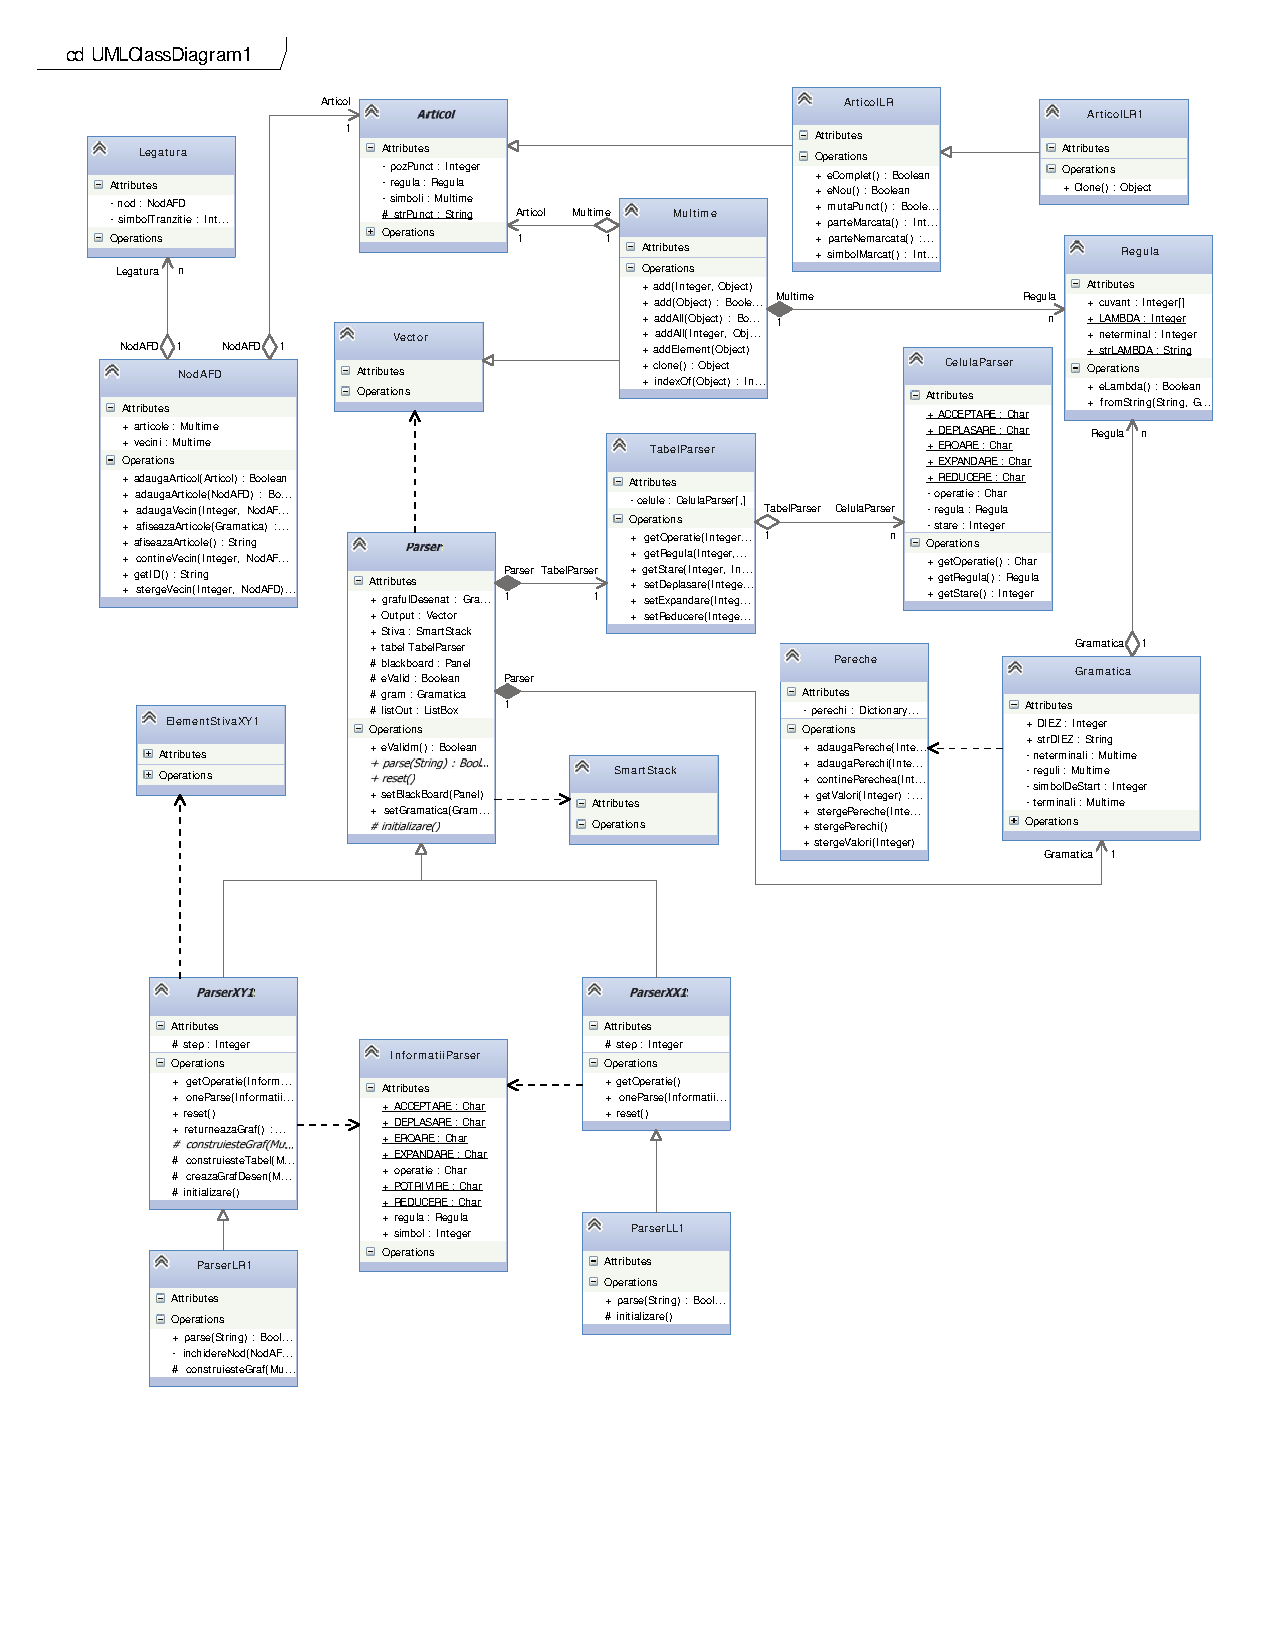
\includegraphics[scale=0.8]{UMLClassDiagram1.pdf} 
%Chapter5
%concluziile (ce am facut)
\chapter{Concluzii}
 
%\input{./Chapters/Chapter6} 
%\input{./Chapters/Chapter7} 

%----------------------------------------------------------------------------------------
%	THESIS CONTENT - APPENDICES
%----------------------------------------------------------------------------------------

\addtocontents{toc}{\vspace{2em}} % Add a gap in the Contents, for aesthetics

\appendix % Cue to tell LaTeX that the following 'chapters' are Appendices

% Include the appendices of the thesis as separate files from the Appendices folder
% Uncomment the lines as you write the Appendices

%% Appendix A

\chapter{Anexa 1} % Main appendix title

\label{AppendixA} % For referencing this appendix elsewhere, use \ref{AppendixA}

\lhead{Appendix A. \emph{Appendix Title Here}} % This is for the header on each page - perhaps a shortened title

Aici trec tot codul
%\input{./Appendices/AppendixB}
%\input{./Appendices/AppendixC}

\addtocontents{toc}{\vspace{2em}} % Add a gap in the Contents, for aesthetics

\backmatter

%----------------------------------------------------------------------------------------
%	LIST OF CONTENTS/FIGURES/TABLES PAGES
%----------------------------------------------------------------------------------------

\pagestyle{fancy} % The page style headers have been "empty" all this time, now use the "fancy" headers as defined before to bring them back

%\lhead{\emph{Contents}} % Set the left side page header to "Contents"
%\tableofcontents % Write out the Table of Contents

\lhead{\emph{List\v a imagini}} % Set the left side page header to "List of Figures"
\listoffigures % Write out the List of Figures

%\lhead{\emph{List of Tables}} % Set the left side page header to "List of Tables"
%\listoftables % Write out the List of Tables



%----------------------------------------------------------------------------------------
%	BIBLIOGRAPHY
%----------------------------------------------------------------------------------------

%\label{Bibliography}

%\lhead{\emph{Bibliography}} % Change the page header to say "Bibliography"

%\bibliographystyle{unsrtnat} % Use the "unsrtnat" BibTeX style for formatting the Bibliography

%\bibliography{Bibliography} % The references (bibliography) information are stored in the file named "Bibliography.bib"


\end{document}  